%%%%%%%%%%%%%%%%%%%%%%%%%%%%%%%%%%%%%%%%%%%%%%%%%%%%%%%%%%%%
% 1.16 CATEGORY THEORY
% The Composition of Advanced Mathematics
%%%%%%%%%%%%%%%%%%%%%%%%%%%%%%%%%%%%%%%%%%%%%%%%%%%%%%%%%%%%

\section{Category Theory}
\label{sec:category-theory}

\prerequisite{
Functions and composition from \cref{sec:functions}, relations from
\cref{sec:relations}, abstract algebra from \cref{sec:abstract-algebra},
group theory from \cref{sec:group-theory}, ring theory from
\cref{sec:ring-theory}, module theory from \cref{sec:module-theory},
universal algebra from \cref{sec:universal-algebra}, and lattice theory from
\cref{sec:lattice-theory}.
}

\learningobjectives{
By the end of this section, the reader should be able to:
\begin{itemize}
    \item explain why category theory studies mathematical structures through
    objects and structure-preserving maps;
    \item define categories, objects, morphisms, identities, and composition;
    \item interpret standard examples such as \(\mathbf{Set}\),
    \(\mathbf{Grp}\), \(\mathbf{Ring}\), and \(\mathbf{Vect}_F\);
    \item recognize isomorphisms, monomorphisms, and epimorphisms;
    \item distinguish initial, terminal, and zero objects;
    \item construct product and coproduct objects through universal properties;
    \item define functors and natural transformations;
    \item distinguish covariant and contravariant constructions;
    \item interpret opposite categories;
    \item understand equivalence of categories;
    \item explain the basic idea of representable functors;
    \item state the Yoneda lemma and explain its conceptual significance;
    \item define adjunctions and recognize their relation to universal
    constructions;
    \item understand limits and colimits as generalizations of familiar
    constructions;
    \item identify the role of category theory throughout modern mathematics.
\end{itemize}
}

%%%%%%%%%%%%%%%%%%%%%%%%%%%%%%%%%%%%%%%%%%%%%%%%%%%%%%%%%%%%
\subsection{Why Category Theory?}
\label{subsec:why-category-theory}
%%%%%%%%%%%%%%%%%%%%%%%%%%%%%%%%%%%%%%%%%%%%%%%%%%%%%%%%%%%%

Much of mathematics studies objects equipped with structure.

Examples include:

\begin{itemize}
    \item sets;
    \item groups;
    \item rings;
    \item fields;
    \item vector spaces;
    \item modules;
    \item topological spaces;
    \item partially ordered sets;
    \item graphs;
    \item manifolds.
\end{itemize}

For each kind of object, mathematics also studies maps that preserve the
relevant structure.

\begin{center}
\begin{tabularx}{0.92\textwidth}{@{}lX@{}}
\toprule
\textbf{Objects} & \textbf{Structure-Preserving Maps}\\
\midrule
Sets & functions\\
Groups & group homomorphisms\\
Rings & ring homomorphisms\\
Vector spaces & linear transformations\\
Modules & module homomorphisms\\
Topological spaces & continuous maps\\
Posets & order-preserving maps\\
\bottomrule
\end{tabularx}
\end{center}

Category theory studies the common structure behind these situations.

\begin{conceptbox}
Category theory shifts attention from the internal elements of mathematical
objects to the relationships among objects expressed through maps.
\end{conceptbox}

This perspective makes it possible to identify patterns that occur
simultaneously throughout algebra, topology, geometry, analysis, logic, and
other branches of mathematics.

%%%%%%%%%%%%%%%%%%%%%%%%%%%%%%%%%%%%%%%%%%%%%%%%%%%%%%%%%%%%
\subsection{Objects and Morphisms}
\label{subsec:objects-morphisms}
%%%%%%%%%%%%%%%%%%%%%%%%%%%%%%%%%%%%%%%%%%%%%%%%%%%%%%%%%%%%

The two basic ingredients of a category are \emph{objects} and
\emph{morphisms}.

A morphism is an abstract arrow between objects.

If \(A\) and \(B\) are objects, a morphism from \(A\) to \(B\) is written

\[ f:A\to B. \]

This is read ``\(f\) is a morphism from \(A\) to \(B\).''

The word \emph{morphism} comes from the idea of a structure-preserving map,
although morphisms in an abstract category need not literally be functions.

%%%%%%%%%%%%%%%%%%%%%%%%%%%%%%%%%%%%%%%%%%%%%%%%%%%%%%%%%%%%
\subsection{Definition of a Category}
\label{subsec:category-definition}
%%%%%%%%%%%%%%%%%%%%%%%%%%%%%%%%%%%%%%%%%%%%%%%%%%%%%%%%%%%%

\begin{definitionbox}{Category}
A \emph{category} \(\mathcal C\) consists of:
\begin{enumerate}
    \item a collection of objects;
    \item for each pair of objects \(A,B\), a collection of morphisms
    from \(A\) to \(B\);
    \item for every object \(A\), an identity morphism
    \[ 1_A:A\to A; \]
    \item a composition operation for compatible morphisms.
\end{enumerate}
Composition must be associative and identity morphisms must act as identities.
\end{definitionbox}

The symbol

\[ \mathcal C \]

is a calligraphic capital \(C\), commonly used to denote a category.

%%%%%%%%%%%%%%%%%%%%%%%%%%%%%%%%%%%%%%%%%%%%%%%%%%%%%%%%%%%%
\subsection{Hom-Sets}
\label{subsec:hom-sets}
%%%%%%%%%%%%%%%%%%%%%%%%%%%%%%%%%%%%%%%%%%%%%%%%%%%%%%%%%%%%

The collection of morphisms from \(A\) to \(B\) is commonly denoted

\[ \operatorname{Hom}_{\mathcal C}(A,B). \]

This is read ``Hom from \(A\) to \(B\) in the category \(\mathcal C\).''

When the category is understood, one often writes simply

\[ \operatorname{Hom}(A,B). \]

Thus

\[ f\in\operatorname{Hom}_{\mathcal C}(A,B) \]

means that \(f\) is a morphism

\[ f:A\to B. \]

%%%%%%%%%%%%%%%%%%%%%%%%%%%%%%%%%%%%%%%%%%%%%%%%%%%%%%%%%%%%
\subsection{Composition}
\label{subsec:categorical-composition}
%%%%%%%%%%%%%%%%%%%%%%%%%%%%%%%%%%%%%%%%%%%%%%%%%%%%%%%%%%%%

Suppose

\[ f:A\to B,\qquad g:B\to C. \]

Then their composite is a morphism

\[ g\circ f:A\to C. \]

The expression

\[ g\circ f \]

is read ``\(g\) composed with \(f\).''

As with ordinary function composition, the map \(f\) acts first and \(g\)
acts second.

\begin{center}
\begin{tikzcd}
A \arrow[r,"f"] \arrow[rr,bend right=25,"g\circ f"'] &
B \arrow[r,"g"] &
C
\end{tikzcd}
\end{center}

%%%%%%%%%%%%%%%%%%%%%%%%%%%%%%%%%%%%%%%%%%%%%%%%%%%%%%%%%%%%
\subsection{Associativity of Composition}
\label{subsec:category-associativity}
%%%%%%%%%%%%%%%%%%%%%%%%%%%%%%%%%%%%%%%%%%%%%%%%%%%%%%%%%%%%

If

\[ f:A\to B,\qquad g:B\to C,\qquad h:C\to D, \]

then category composition must satisfy

\[ h\circ(g\circ f)=(h\circ g)\circ f. \]

Therefore an unambiguous composite may be written

\[ h\circ g\circ f. \]

Diagrammatically,

\begin{center}
\begin{tikzcd}
A \arrow[r,"f"] &
B \arrow[r,"g"] &
C \arrow[r,"h"] &
D
\end{tikzcd}
\end{center}

both possible parenthesizations produce the same morphism from \(A\) to
\(D\).

%%%%%%%%%%%%%%%%%%%%%%%%%%%%%%%%%%%%%%%%%%%%%%%%%%%%%%%%%%%%
\subsection{Identity Morphisms}
\label{subsec:identity-morphisms}
%%%%%%%%%%%%%%%%%%%%%%%%%%%%%%%%%%%%%%%%%%%%%%%%%%%%%%%%%%%%

For every object \(A\), there is an identity morphism

\[ 1_A:A\to A. \]

It satisfies

\[ 1_B\circ f=f \]

for every

\[ f:A\to B, \]

and

\[ f\circ1_A=f. \]

Thus identity morphisms behave like identity functions.

Some texts use

\[ \operatorname{id}_A \]

instead of \(1_A\).

This is read ``the identity on \(A\).''

%%%%%%%%%%%%%%%%%%%%%%%%%%%%%%%%%%%%%%%%%%%%%%%%%%%%%%%%%%%%
\subsection{A Category as a Network}
\label{subsec:category-network}
%%%%%%%%%%%%%%%%%%%%%%%%%%%%%%%%%%%%%%%%%%%%%%%%%%%%%%%%%%%%

A useful first picture of a category is a network of objects connected by
morphisms.

\begin{center}
\begin{tikzcd}[column sep=large,row sep=large]
A \arrow[r,bend left=15,"f"] \arrow[dr,"h"'] &
B \arrow[l,bend left=15,"g"] \arrow[d,"k"]\\
&
C
\end{tikzcd}
\end{center}

The objects are nodes.

The morphisms are arrows.

Unlike an ordinary graph, however, a category also contains composites of
compatible arrows and an identity arrow at every object.

%%%%%%%%%%%%%%%%%%%%%%%%%%%%%%%%%%%%%%%%%%%%%%%%%%%%%%%%%%%%
\subsection{The Category of Sets}
\label{subsec:category-set}
%%%%%%%%%%%%%%%%%%%%%%%%%%%%%%%%%%%%%%%%%%%%%%%%%%%%%%%%%%%%

The most familiar category is

\[ \mathbf{Set}. \]

Its objects are sets and its morphisms are functions.

Thus if \(A\) and \(B\) are sets,

\[ \operatorname{Hom}_{\mathbf{Set}}(A,B) \]

is the collection of functions from \(A\) to \(B\).

Composition is ordinary function composition, and the identity morphism is
the ordinary identity function.

%%%%%%%%%%%%%%%%%%%%%%%%%%%%%%%%%%%%%%%%%%%%%%%%%%%%%%%%%%%%
\subsection{The Category of Groups}
\label{subsec:category-grp}
%%%%%%%%%%%%%%%%%%%%%%%%%%%%%%%%%%%%%%%%%%%%%%%%%%%%%%%%%%%%

The category

\[ \mathbf{Grp} \]

has:

\begin{itemize}
    \item groups as objects;
    \item group homomorphisms as morphisms.
\end{itemize}

Thus

\[ \operatorname{Hom}_{\mathbf{Grp}}(G,H) \]

is the set of group homomorphisms

\[ G\to H. \]

The composition of group homomorphisms is again a group homomorphism.

%%%%%%%%%%%%%%%%%%%%%%%%%%%%%%%%%%%%%%%%%%%%%%%%%%%%%%%%%%%%
\subsection{Other Algebraic Categories}
\label{subsec:algebraic-categories}
%%%%%%%%%%%%%%%%%%%%%%%%%%%%%%%%%%%%%%%%%%%%%%%%%%%%%%%%%%%%

Many algebraic structures naturally form categories.

\begin{center}
\begin{tabularx}{0.92\textwidth}{@{}lXX@{}}
\toprule
\textbf{Category} & \textbf{Objects} & \textbf{Morphisms}\\
\midrule
\(\mathbf{Ring}\) & rings & ring homomorphisms\\
\(\mathbf{Field}\) & fields & field homomorphisms\\
\(R\text{-}\mathbf{Mod}\) & left \(R\)-modules & \(R\)-module homomorphisms\\
\(\mathbf{Vect}_F\) & vector spaces over \(F\) & \(F\)-linear maps\\
\(\mathbf{Ab}\) & abelian groups & group homomorphisms\\
\(\mathbf{Lat}\) & lattices & lattice homomorphisms\\
\bottomrule
\end{tabularx}
\end{center}

Notation varies among authors, but the underlying idea is the same.

%%%%%%%%%%%%%%%%%%%%%%%%%%%%%%%%%%%%%%%%%%%%%%%%%%%%%%%%%%%%
\subsection{The Category of Topological Spaces}
\label{subsec:category-top}
%%%%%%%%%%%%%%%%%%%%%%%%%%%%%%%%%%%%%%%%%%%%%%%%%%%%%%%%%%%%

The category

\[ \mathbf{Top} \]

has topological spaces as objects and continuous functions as morphisms.

This example demonstrates that category theory is not restricted to algebra.

Later chapters will use categorical ideas to organize constructions in
topology, geometry, and analysis.

%%%%%%%%%%%%%%%%%%%%%%%%%%%%%%%%%%%%%%%%%%%%%%%%%%%%%%%%%%%%
\subsection{Posets as Categories}
\label{subsec:posets-as-categories}
%%%%%%%%%%%%%%%%%%%%%%%%%%%%%%%%%%%%%%%%%%%%%%%%%%%%%%%%%%%%

Every poset

\[ (P,\leq) \]

can be regarded as a category.

The elements of \(P\) are objects.

There is a unique morphism

\[ x\to y \]

exactly when

\[ x\leq y. \]

Reflexivity supplies identity morphisms, and transitivity supplies
composition.

\begin{center}
\begin{tikzcd}
x \arrow[r] & y \arrow[r] & z
\end{tikzcd}
\end{center}

corresponds to

\[ x\leq y\leq z, \]

which implies

\[ x\leq z. \]

This explains why many order-theoretic ideas have categorical analogues.

%%%%%%%%%%%%%%%%%%%%%%%%%%%%%%%%%%%%%%%%%%%%%%%%%%%%%%%%%%%%
\subsection{Groups as One-Object Categories}
\label{subsec:groups-one-object-category}
%%%%%%%%%%%%%%%%%%%%%%%%%%%%%%%%%%%%%%%%%%%%%%%%%%%%%%%%%%%%

A group can also be interpreted categorically.

Take a category with one object, say \(*\).

Let the morphisms

\[ *\to* \]

be the elements of a group \(G\).

Composition is group multiplication.

The identity morphism is the group identity.

Because every group element has an inverse, every morphism is invertible.

\begin{conceptbox}
A group can be viewed as a category with exactly one object in which every
morphism is an isomorphism.
\end{conceptbox}

This is an important example of how category theory reorganizes familiar
algebraic structures.

%%%%%%%%%%%%%%%%%%%%%%%%%%%%%%%%%%%%%%%%%%%%%%%%%%%%%%%%%%%%
\subsection{Isomorphisms}
\label{subsec:categorical-isomorphisms}
%%%%%%%%%%%%%%%%%%%%%%%%%%%%%%%%%%%%%%%%%%%%%%%%%%%%%%%%%%%%

\begin{definitionbox}{Isomorphism}
A morphism
\[ f:A\to B \]
is an \emph{isomorphism} if there exists a morphism
\[ g:B\to A \]
such that
\[ g\circ f=1_A,\qquad f\circ g=1_B. \]
\end{definitionbox}

The morphism \(g\) is the inverse of \(f\).

One writes

\[ A\cong B \]

when \(A\) and \(B\) are isomorphic.

%%%%%%%%%%%%%%%%%%%%%%%%%%%%%%%%%%%%%%%%%%%%%%%%%%%%%%%%%%%%
\subsection{Isomorphism Diagram}
\label{subsec:isomorphism-diagram}
%%%%%%%%%%%%%%%%%%%%%%%%%%%%%%%%%%%%%%%%%%%%%%%%%%%%%%%%%%%%

An isomorphism may be visualized as

\begin{center}
\begin{tikzcd}[column sep=huge]
A \arrow[r,bend left=18,"f"] &
B \arrow[l,bend left=18,"g"]
\end{tikzcd}
\end{center}

with

\[ g\circ f=1_A,\qquad f\circ g=1_B. \]

Categorically, isomorphic objects possess the same structure relevant to the
category.

%%%%%%%%%%%%%%%%%%%%%%%%%%%%%%%%%%%%%%%%%%%%%%%%%%%%%%%%%%%%
\subsection{Isomorphism Versus Equality}
\label{subsec:isomorphism-versus-equality}
%%%%%%%%%%%%%%%%%%%%%%%%%%%%%%%%%%%%%%%%%%%%%%%%%%%%%%%%%%%%

Two objects can be isomorphic without being literally equal.

For example, the sets

\[ A=\{1,2,3\},\qquad B=\{a,b,c\} \]

are different sets but are isomorphic in \(\mathbf{Set}\) because there is
a bijection between them.

Likewise, two vector spaces may contain completely different elements yet
be isomorphic as vector spaces.

\begin{importantbox}
Category theory generally treats isomorphic objects as structurally
equivalent even when they are not literally identical.
\end{importantbox}

%%%%%%%%%%%%%%%%%%%%%%%%%%%%%%%%%%%%%%%%%%%%%%%%%%%%%%%%%%%%
\subsection{Monomorphisms}
\label{subsec:monomorphisms}
%%%%%%%%%%%%%%%%%%%%%%%%%%%%%%%%%%%%%%%%%%%%%%%%%%%%%%%%%%%%

Category theory generalizes injectivity without referring directly to
elements.

\begin{definitionbox}{Monomorphism}
A morphism
\[ f:A\to B \]
is a \emph{monomorphism} if for every pair
\[ g,h:X\to A, \]
the equality
\[ f\circ g=f\circ h \]
implies
\[ g=h. \]
\end{definitionbox}

A monomorphism is often abbreviated \emph{mono}.

It is sometimes written

\[ A\hookrightarrow B. \]

The hooked arrow \(\hookrightarrow\) often suggests an injective or
embedding-like morphism, although notation depends on context.

%%%%%%%%%%%%%%%%%%%%%%%%%%%%%%%%%%%%%%%%%%%%%%%%%%%%%%%%%%%%
\subsection{Epimorphisms}
\label{subsec:epimorphisms}
%%%%%%%%%%%%%%%%%%%%%%%%%%%%%%%%%%%%%%%%%%%%%%%%%%%%%%%%%%%%

The dual concept is an epimorphism.

\begin{definitionbox}{Epimorphism}
A morphism
\[ f:A\to B \]
is an \emph{epimorphism} if for every pair
\[ g,h:B\to X, \]
the equality
\[ g\circ f=h\circ f \]
implies
\[ g=h. \]
\end{definitionbox}

An epimorphism is often abbreviated \emph{epi}.

A common notation is

\[ A\twoheadrightarrow B. \]

The double-headed arrow \(\twoheadrightarrow\) commonly indicates a
surjective or quotient-like morphism.

%%%%%%%%%%%%%%%%%%%%%%%%%%%%%%%%%%%%%%%%%%%%%%%%%%%%%%%%%%%%
\subsection{Cancellation Interpretation}
\label{subsec:categorical-cancellation}
%%%%%%%%%%%%%%%%%%%%%%%%%%%%%%%%%%%%%%%%%%%%%%%%%%%%%%%%%%%%

Monomorphisms and epimorphisms can be remembered through cancellation.

A monomorphism permits left cancellation:

\[ f\circ g=f\circ h\Longrightarrow g=h. \]

An epimorphism permits right cancellation:

\[ g\circ f=h\circ f\Longrightarrow g=h. \]

\begin{center}
\begin{tikzcd}[column sep=large]
X \arrow[r,shift left=3pt,"g"] \arrow[r,shift right=3pt,"h"'] &
A \arrow[r,"f"] &
B
\end{tikzcd}
\end{center}

If \(f\) is monic, equality after composing with \(f\) forces \(g=h\).

%%%%%%%%%%%%%%%%%%%%%%%%%%%%%%%%%%%%%%%%%%%%%%%%%%%%%%%%%%%%
\subsection{Monic Does Not Always Mean Injective}
\label{subsec:monic-not-injective}
%%%%%%%%%%%%%%%%%%%%%%%%%%%%%%%%%%%%%%%%%%%%%%%%%%%%%%%%%%%%

In \(\mathbf{Set}\), monomorphisms are exactly injective functions.

In many familiar algebraic categories, monomorphisms are also injective
homomorphisms.

However, the categorical definition does not mention elements.

Similarly, epimorphisms need not always be surjective.

For example, in the category of rings with identity and identity-preserving
homomorphisms, the inclusion

\[ \Z\hookrightarrow\Q \]

is an epimorphism even though it is not surjective.

This illustrates why categorical concepts must be understood through their
universal behavior rather than only through familiar set-theoretic models.

%%%%%%%%%%%%%%%%%%%%%%%%%%%%%%%%%%%%%%%%%%%%%%%%%%%%%%%%%%%%
\subsection{Initial Objects}
\label{subsec:initial-objects}
%%%%%%%%%%%%%%%%%%%%%%%%%%%%%%%%%%%%%%%%%%%%%%%%%%%%%%%%%%%%

\begin{definitionbox}{Initial Object}
An object \(I\) in a category \(\mathcal C\) is \emph{initial} if for every
object \(A\), there exists exactly one morphism
\[ I\to A. \]
\end{definitionbox}

Diagrammatically,

\begin{center}
\begin{tikzcd}
I \arrow[r,dashed,"\exists!"'] & A
\end{tikzcd}
\end{center}

The symbol

\[ \exists! \]

is read ``there exists a unique.''

In \(\mathbf{Set}\), the empty set

\[ \varnothing \]

is initial because there is exactly one function

\[ \varnothing\to A \]

for every set \(A\).

%%%%%%%%%%%%%%%%%%%%%%%%%%%%%%%%%%%%%%%%%%%%%%%%%%%%%%%%%%%%
\subsection{Terminal Objects}
\label{subsec:terminal-objects}
%%%%%%%%%%%%%%%%%%%%%%%%%%%%%%%%%%%%%%%%%%%%%%%%%%%%%%%%%%%%

\begin{definitionbox}{Terminal Object}
An object \(T\) is \emph{terminal} if for every object \(A\), there exists
exactly one morphism
\[ A\to T. \]
\end{definitionbox}

In \(\mathbf{Set}\), every singleton set is terminal.

If

\[ T=\{*\}, \]

then every set \(A\) has exactly one function

\[ A\to\{*\}. \]

It sends every element of \(A\) to \(*\).

%%%%%%%%%%%%%%%%%%%%%%%%%%%%%%%%%%%%%%%%%%%%%%%%%%%%%%%%%%%%
\subsection{Uniqueness up to Unique Isomorphism}
\label{subsec:unique-up-to-isomorphism}
%%%%%%%%%%%%%%%%%%%%%%%%%%%%%%%%%%%%%%%%%%%%%%%%%%%%%%%%%%%%

Initial and terminal objects need not be literally unique.

Instead, they satisfy a stronger structural principle.

\begin{theorem}
Any two initial objects in a category are uniquely isomorphic.
Likewise, any two terminal objects are uniquely isomorphic.
\end{theorem}

\begin{proof}
Let \(I\) and \(J\) be initial.

Since \(I\) is initial, there is a unique morphism

\[ f:I\to J. \]

Since \(J\) is initial, there is a unique morphism

\[ g:J\to I. \]

Then

\[ g\circ f:I\to I. \]

But there is exactly one morphism \(I\to I\), and \(1_I\) is such a
morphism. Hence

\[ g\circ f=1_I. \]

Similarly,

\[ f\circ g=1_J. \]

Therefore \(I\cong J\).
\end{proof}

%%%%%%%%%%%%%%%%%%%%%%%%%%%%%%%%%%%%%%%%%%%%%%%%%%%%%%%%%%%%
\subsection{Zero Objects}
\label{subsec:zero-objects}
%%%%%%%%%%%%%%%%%%%%%%%%%%%%%%%%%%%%%%%%%%%%%%%%%%%%%%%%%%%%

\begin{definitionbox}{Zero Object}
An object is a \emph{zero object} if it is both initial and terminal.
\end{definitionbox}

A zero object is commonly denoted

\[ 0. \]

In \(\mathbf{Grp}\), the trivial group is a zero object.

In \(\mathbf{Vect}_F\), the zero vector space is a zero object.

The category \(\mathbf{Set}\) does not have a zero object because the empty
set is initial but not terminal.

%%%%%%%%%%%%%%%%%%%%%%%%%%%%%%%%%%%%%%%%%%%%%%%%%%%%%%%%%%%%
\subsection{Universal Properties}
\label{subsec:universal-properties}
%%%%%%%%%%%%%%%%%%%%%%%%%%%%%%%%%%%%%%%%%%%%%%%%%%%%%%%%%%%%

One of the central ideas of category theory is the \emph{universal
property}.

Instead of describing an object solely through its internal construction,
one characterizes it through the unique maps connecting it to all relevant
objects.

\begin{conceptbox}
A universal property describes a mathematical object by how morphisms
uniquely factor through it.
\end{conceptbox}

Initial objects and terminal objects are the simplest examples.

Products, coproducts, kernels, quotients, tensor products, free objects, and
many other constructions can also be described universally.

%%%%%%%%%%%%%%%%%%%%%%%%%%%%%%%%%%%%%%%%%%%%%%%%%%%%%%%%%%%%
\subsection{Categorical Products}
\label{subsec:categorical-products}
%%%%%%%%%%%%%%%%%%%%%%%%%%%%%%%%%%%%%%%%%%%%%%%%%%%%%%%%%%%%

\begin{definitionbox}{Product}
A \emph{product} of objects \(A\) and \(B\) is an object \(A\times B\)
together with morphisms
\[ \pi_A:A\times B\to A,\qquad
\pi_B:A\times B\to B \]
such that for every object \(X\) with morphisms
\[ f:X\to A,\qquad g:X\to B, \]
there exists a unique morphism
\[ \langle f,g\rangle:X\to A\times B \]
making the corresponding diagram commute.
\end{definitionbox}

The lowercase Greek letter

\[ \pi \]

is \emph{pi}, pronounced ``pie.''

Here \(\pi_A\) and \(\pi_B\) are called projection morphisms.

%%%%%%%%%%%%%%%%%%%%%%%%%%%%%%%%%%%%%%%%%%%%%%%%%%%%%%%%%%%%
\subsection{Product Universal Diagram}
\label{subsec:product-universal-diagram}
%%%%%%%%%%%%%%%%%%%%%%%%%%%%%%%%%%%%%%%%%%%%%%%%%%%%%%%%%%%%

The defining diagram is

\begin{centereddiagram}
\begin{tikzcd}[column sep=large,row sep=large]
& X \arrow[dl,"f"'] \arrow[d,dashed,"{\exists!\,\langle f,g\rangle}"] \arrow[dr,"g"] & \\
A & A\times B \arrow[l,"\pi_A"] \arrow[r,"\pi_B"'] & B
\end{tikzcd}
\end{centereddiagram}

Commutativity means

\[ \pi_A\circ\langle f,g\rangle=f, \]

and

\[ \pi_B\circ\langle f,g\rangle=g. \]

The universal property determines the product uniquely up to unique
isomorphism.

%%%%%%%%%%%%%%%%%%%%%%%%%%%%%%%%%%%%%%%%%%%%%%%%%%%%%%%%%%%%
\subsection{Products in Familiar Categories}
\label{subsec:products-familiar-categories}
%%%%%%%%%%%%%%%%%%%%%%%%%%%%%%%%%%%%%%%%%%%%%%%%%%%%%%%%%%%%

In \(\mathbf{Set}\), the categorical product is the Cartesian product.

In \(\mathbf{Grp}\), it is the direct product of groups.

In \(\mathbf{Vect}_F\), the product of finitely many vector spaces agrees
with their direct sum.

Thus several familiar constructions are instances of one categorical idea.

%%%%%%%%%%%%%%%%%%%%%%%%%%%%%%%%%%%%%%%%%%%%%%%%%%%%%%%%%%%%
\subsection{Coproducts}
\label{subsec:categorical-coproducts}
%%%%%%%%%%%%%%%%%%%%%%%%%%%%%%%%%%%%%%%%%%%%%%%%%%%%%%%%%%%%

The dual construction is the coproduct.

\begin{definitionbox}{Coproduct}
A \emph{coproduct} of \(A\) and \(B\) is an object \(A\amalg B\) equipped
with morphisms
\[ \iota_A:A\to A\amalg B,\qquad
\iota_B:B\to A\amalg B \]
such that for every pair
\[ f:A\to X,\qquad g:B\to X, \]
there exists a unique morphism
\[ [f,g]:A\amalg B\to X \]
making the defining diagram commute.
\end{definitionbox}

The symbol

\[ \amalg \]

is often read ``coproduct'' or ``disjoint union.''

The lowercase Greek letter

\[ \iota \]

is \emph{iota}, pronounced ``eye-oh-tuh.''

%%%%%%%%%%%%%%%%%%%%%%%%%%%%%%%%%%%%%%%%%%%%%%%%%%%%%%%%%%%%
\subsection{Coproduct Universal Diagram}
\label{subsec:coproduct-universal-diagram}
%%%%%%%%%%%%%%%%%%%%%%%%%%%%%%%%%%%%%%%%%%%%%%%%%%%%%%%%%%%%

\begin{centereddiagram}
\begin{tikzcd}[column sep=large,row sep=large]
A \arrow[r,"\iota_A"] \arrow[dr,"f"'] &
A\amalg B \arrow[d,dashed,"{\exists!\,[f,g]}"] &
B \arrow[l,"\iota_B"'] \arrow[dl,"g"]\\
& X &
\end{tikzcd}
\end{centereddiagram}

The diagram commutes when

\[ [f,g]\circ\iota_A=f, \]

and

\[ [f,g]\circ\iota_B=g. \]
%%%%%%%%%%%%%%%%%%%%%%%%%%%%%%%%%%%%%%%%%%%%%%%%%%%%%%%%%%%%
\subsection{Coproducts in Familiar Categories}
\label{subsec:coproducts-familiar}
%%%%%%%%%%%%%%%%%%%%%%%%%%%%%%%%%%%%%%%%%%%%%%%%%%%%%%%%%%%%

Coproducts depend strongly on the category.

\begin{center}
\begin{tabularx}{0.9\textwidth}{@{}lX@{}}
\toprule
\textbf{Category} & \textbf{Coproduct}\\
\midrule
\(\mathbf{Set}\) & disjoint union\\
\(\mathbf{Grp}\) & free product\\
\(\mathbf{Ab}\) & direct sum\\
\(\mathbf{Vect}_F\) & direct sum\\
\bottomrule
\end{tabularx}
\end{center}

The same universal pattern therefore produces different concrete
constructions in different categories.

%%%%%%%%%%%%%%%%%%%%%%%%%%%%%%%%%%%%%%%%%%%%%%%%%%%%%%%%%%%%
\subsection{Worked Example: Product in \(\mathbf{Set}\)}
\label{subsec:worked-category-product}
%%%%%%%%%%%%%%%%%%%%%%%%%%%%%%%%%%%%%%%%%%%%%%%%%%%%%%%%%%%%

\begin{workedexamplebox}{The Cartesian Product as a Categorical Product}

Let \(A\) and \(B\) be sets and suppose

\[ f:X\to A,\qquad g:X\to B. \]

Construct the unique map \(X\to A\times B\).

\begin{tabularx}{\textwidth}{@{}>{\raggedright\arraybackslash}p{0.42\textwidth}X@{}}
The map must remember both \(f(x)\) and \(g(x)\). &
\(h(x)=(f(x),g(x))\)\\
Projecting to \(A\) recovers \(f\). &
\(\pi_A(h(x))=f(x)\)\\
Projecting to \(B\) recovers \(g\). &
\(\pi_B(h(x))=g(x)\)\\
Any map satisfying both conditions must have these coordinates. &
\(h=\langle f,g\rangle\)
\end{tabularx}

\begin{answerbox}
\[ \boxed{\langle f,g\rangle(x)=(f(x),g(x)).} \]
\end{answerbox}
\end{workedexamplebox}

%%%%%%%%%%%%%%%%%%%%%%%%%%%%%%%%%%%%%%%%%%%%%%%%%%%%%%%%%%%%
\subsection{Commutative Diagrams}
\label{subsec:commutative-diagrams}
%%%%%%%%%%%%%%%%%%%%%%%%%%%%%%%%%%%%%%%%%%%%%%%%%%%%%%%%%%%%

Category theory frequently expresses equations through diagrams.

A diagram is \emph{commutative} if every directed path with the same starting
and ending objects gives the same composite morphism.

For example,

\begin{center}
\begin{tikzcd}[column sep=large,row sep=large]
A \arrow[r,"f"] \arrow[dr,"h"'] &
B \arrow[d,"g"]\\
& C
\end{tikzcd}
\end{center}

commutes when

\[ g\circ f=h. \]

Commutative diagrams allow large collections of equations to be represented
visually.

%%%%%%%%%%%%%%%%%%%%%%%%%%%%%%%%%%%%%%%%%%%%%%%%%%%%%%%%%%%%
\subsection{Functors}
\label{subsec:functors}
%%%%%%%%%%%%%%%%%%%%%%%%%%%%%%%%%%%%%%%%%%%%%%%%%%%%%%%%%%%%

Categories themselves can be related by structure-preserving maps.

These are called functors.

\begin{definitionbox}{Covariant Functor}
A \emph{covariant functor}
\[ F:\mathcal C\to\mathcal D \]
assigns:
\begin{itemize}
    \item to every object \(A\) of \(\mathcal C\), an object \(F(A)\) of
    \(\mathcal D\);
    \item to every morphism \(f:A\to B\), a morphism
    \[ F(f):F(A)\to F(B), \]
\end{itemize}
such that identities and composition are preserved.
\end{definitionbox}

Thus

\[ F(1_A)=1_{F(A)}, \]

and

\[ F(g\circ f)=F(g)\circ F(f). \]

%%%%%%%%%%%%%%%%%%%%%%%%%%%%%%%%%%%%%%%%%%%%%%%%%%%%%%%%%%%%
\subsection{Visualizing a Functor}
\label{subsec:functor-visual}
%%%%%%%%%%%%%%%%%%%%%%%%%%%%%%%%%%%%%%%%%%%%%%%%%%%%%%%%%%%%

A functor transports an entire diagram from one category to another.

\begin{center}
\begin{tikzpicture}[
    box/.style={draw,rounded corners,minimum width=36mm,minimum height=28mm},
    >=stealth
]
\node[box] (C) at (0,0) {\(\mathcal C:\quad A\xrightarrow{f}B\)};
\node[box] (D) at (6,0) {\(\mathcal D:\quad F(A)\xrightarrow{F(f)}F(B)\)};
\draw[->,thick] (C)--node[above]{\(F\)}(D);
\end{tikzpicture}
\end{center}

The essential point is that the pattern of composition is preserved.

%%%%%%%%%%%%%%%%%%%%%%%%%%%%%%%%%%%%%%%%%%%%%%%%%%%%%%%%%%%%
\subsection{Forgetful Functors}
\label{subsec:forgetful-functors}
%%%%%%%%%%%%%%%%%%%%%%%%%%%%%%%%%%%%%%%%%%%%%%%%%%%%%%%%%%%%

A common functor discards some structure.

For example,

\[ U:\mathbf{Grp}\to\mathbf{Set} \]

sends each group to its underlying set and each group homomorphism to its
underlying function.

The letter \(U\) commonly suggests \emph{underlying} or \emph{forgetful}.

Similarly,

\[ U:\mathbf{Vect}_F\to\mathbf{Set} \]

forgets the vector-space operations and remembers only the underlying set.

%%%%%%%%%%%%%%%%%%%%%%%%%%%%%%%%%%%%%%%%%%%%%%%%%%%%%%%%%%%%
\subsection{Free Constructions as Functors}
\label{subsec:free-functors}
%%%%%%%%%%%%%%%%%%%%%%%%%%%%%%%%%%%%%%%%%%%%%%%%%%%%%%%%%%%%

A set \(X\) can be sent to the free group generated by \(X\).

This defines a functor

\[ F:\mathbf{Set}\to\mathbf{Grp}. \]

Likewise one may construct:

\begin{itemize}
    \item free abelian groups;
    \item free modules;
    \item free associative algebras;
    \item free lattices;
    \item free universal algebras.
\end{itemize}

These constructions are closely related to adjunctions.

%%%%%%%%%%%%%%%%%%%%%%%%%%%%%%%%%%%%%%%%%%%%%%%%%%%%%%%%%%%%
\subsection{Identity Functor}
\label{subsec:identity-functor}
%%%%%%%%%%%%%%%%%%%%%%%%%%%%%%%%%%%%%%%%%%%%%%%%%%%%%%%%%%%%

Every category \(\mathcal C\) has an identity functor

\[ 1_{\mathcal C}:\mathcal C\to\mathcal C. \]

It sends

\[ A\mapsto A \]

and

\[ f\mapsto f. \]

Functor composition is associative, and identity functors behave as
identities.

Consequently, categories themselves can be organized into higher-level
categorical structures.

%%%%%%%%%%%%%%%%%%%%%%%%%%%%%%%%%%%%%%%%%%%%%%%%%%%%%%%%%%%%
\subsection{Contravariant Functors}
\label{subsec:contravariant-functors}
%%%%%%%%%%%%%%%%%%%%%%%%%%%%%%%%%%%%%%%%%%%%%%%%%%%%%%%%%%%%

Some constructions reverse the direction of morphisms.

\begin{definitionbox}{Contravariant Functor}
A \emph{contravariant functor}
\[ F:\mathcal C\to\mathcal D \]
assigns a morphism
\[ f:A\to B \]
to a morphism
\[ F(f):F(B)\to F(A), \]
reversing the direction of arrows.
\end{definitionbox}

Composition is reversed:

\[ F(g\circ f)=F(f)\circ F(g). \]

%%%%%%%%%%%%%%%%%%%%%%%%%%%%%%%%%%%%%%%%%%%%%%%%%%%%%%%%%%%%
\subsection{Opposite Categories}
\label{subsec:opposite-categories}
%%%%%%%%%%%%%%%%%%%%%%%%%%%%%%%%%%%%%%%%%%%%%%%%%%%%%%%%%%%%

Contravariance can be expressed using an opposite category.

\begin{definitionbox}{Opposite Category}
The \emph{opposite category} \(\mathcal C^{\mathrm{op}}\) has the same
objects as \(\mathcal C\), but every morphism is reversed.
\end{definitionbox}

Thus a morphism

\[ f:A\to B \]

in \(\mathcal C\) becomes a morphism

\[ f^{\mathrm{op}}:B\to A \]

in \(\mathcal C^{\mathrm{op}}\).

The superscript

\[ \mathrm{op} \]

is read ``opposite.''

A contravariant functor from \(\mathcal C\) to \(\mathcal D\) can therefore
be treated as an ordinary covariant functor

\[ F:\mathcal C^{\mathrm{op}}\to\mathcal D. \]

%%%%%%%%%%%%%%%%%%%%%%%%%%%%%%%%%%%%%%%%%%%%%%%%%%%%%%%%%%%%
\subsection{Dual Vector Spaces as a Contravariant Example}
\label{subsec:dual-space-functor}
%%%%%%%%%%%%%%%%%%%%%%%%%%%%%%%%%%%%%%%%%%%%%%%%%%%%%%%%%%%%

Let \(V\) be a vector space over \(F\).

Its dual space is

\[ V^*=\operatorname{Hom}_F(V,F). \]

If

\[ T:V\to W \]

is linear, then the dual map goes in the opposite direction:

\[ T^*:W^*\to V^*. \]

It is defined by

\[ T^*(\varphi)=\varphi\circ T. \]

Thus dualization reverses arrows.

This is a natural example of a contravariant construction.

%%%%%%%%%%%%%%%%%%%%%%%%%%%%%%%%%%%%%%%%%%%%%%%%%%%%%%%%%%%%
\subsection{Natural Transformations}
\label{subsec:natural-transformations}
%%%%%%%%%%%%%%%%%%%%%%%%%%%%%%%%%%%%%%%%%%%%%%%%%%%%%%%%%%%%

Functors are maps between categories.

Natural transformations are maps between functors.

\begin{definitionbox}{Natural Transformation}
Let
\[ F,G:\mathcal C\to\mathcal D \]
be functors. A \emph{natural transformation}
\[ \eta:F\Rightarrow G \]
assigns to every object \(A\) of \(\mathcal C\) a morphism
\[ \eta_A:F(A)\to G(A) \]
such that for every morphism \(f:A\to B\), the naturality square commutes.
\end{definitionbox}

The symbol

\[ \eta \]

is the lowercase Greek letter \emph{eta}, commonly pronounced
``ay-tuh'' or ``ee-tuh.''

The double arrow

\[ \Rightarrow \]

indicates a transformation between functors rather than a morphism between
ordinary objects.

%%%%%%%%%%%%%%%%%%%%%%%%%%%%%%%%%%%%%%%%%%%%%%%%%%%%%%%%%%%%
\subsection{Naturality Square}
\label{subsec:naturality-square}
%%%%%%%%%%%%%%%%%%%%%%%%%%%%%%%%%%%%%%%%%%%%%%%%%%%%%%%%%%%%

The defining condition is represented by

\begin{center}
\begin{tikzcd}[column sep=large,row sep=large]
F(A) \arrow[r,"F(f)"] \arrow[d,"\eta_A"'] &
F(B) \arrow[d,"\eta_B"]\\
G(A) \arrow[r,"G(f)"'] &
G(B)
\end{tikzcd}
\end{center}

Commutativity means

\[ \eta_B\circ F(f)=G(f)\circ\eta_A. \]

The components \(\eta_A\) must therefore interact consistently with every
morphism of \(\mathcal C\).

%%%%%%%%%%%%%%%%%%%%%%%%%%%%%%%%%%%%%%%%%%%%%%%%%%%%%%%%%%%%
\subsection{Natural Isomorphisms}
\label{subsec:natural-isomorphisms}
%%%%%%%%%%%%%%%%%%%%%%%%%%%%%%%%%%%%%%%%%%%%%%%%%%%%%%%%%%%%

A natural transformation

\[ \eta:F\Rightarrow G \]

is a \emph{natural isomorphism} if every component

\[ \eta_A:F(A)\to G(A) \]

is an isomorphism.

One then writes

\[ F\cong G. \]

This means that the two functors perform essentially the same construction
in a way compatible with all morphisms.

%%%%%%%%%%%%%%%%%%%%%%%%%%%%%%%%%%%%%%%%%%%%%%%%%%%%%%%%%%%%
\subsection{A Natural Isomorphism Example}
\label{subsec:natural-isomorphism-example}
%%%%%%%%%%%%%%%%%%%%%%%%%%%%%%%%%%%%%%%%%%%%%%%%%%%%%%%%%%%%

For finite-dimensional vector spaces over \(F\), there is a canonical map

\[ V\to V^{**}. \]

It sends a vector \(v\) to the functional

\[ \widehat v:V^*\to F,\qquad \widehat v(\varphi)=\varphi(v). \]

This construction is natural in \(V\).

Thus finite-dimensional vector spaces are naturally isomorphic to their
double duals.

By contrast, an isomorphism

\[ V\cong V^* \]

usually requires choosing a basis or additional structure and is not
canonical in the same way.

%%%%%%%%%%%%%%%%%%%%%%%%%%%%%%%%%%%%%%%%%%%%%%%%%%%%%%%%%%%%
\subsection{Equivalence of Categories}
\label{subsec:equivalence-categories}
%%%%%%%%%%%%%%%%%%%%%%%%%%%%%%%%%%%%%%%%%%%%%%%%%%%%%%%%%%%%

Two categories may describe essentially the same mathematics without being
literally isomorphic as categories.

\begin{definitionbox}{Equivalence of Categories}
Categories \(\mathcal C\) and \(\mathcal D\) are \emph{equivalent} if there
exist functors
\[ F:\mathcal C\to\mathcal D,\qquad
G:\mathcal D\to\mathcal C \]
together with natural isomorphisms
\[ G\circ F\cong1_{\mathcal C},\qquad
F\circ G\cong1_{\mathcal D}. \]
\end{definitionbox}

One often writes

\[ \mathcal C\simeq\mathcal D. \]

The symbol \(\simeq\) is read ``equivalent to'' in this context.

%%%%%%%%%%%%%%%%%%%%%%%%%%%%%%%%%%%%%%%%%%%%%%%%%%%%%%%%%%%%
\subsection{Isomorphism Versus Equivalence of Categories}
\label{subsec:isomorphism-equivalence-categories}
%%%%%%%%%%%%%%%%%%%%%%%%%%%%%%%%%%%%%%%%%%%%%%%%%%%%%%%%%%%%

An isomorphism of categories requires exact inverse functors.

An equivalence allows the composites to be naturally isomorphic to the
identity functors.

Thus equivalence is weaker than literal categorical isomorphism but captures
the notion of having the same categorical structure.

\begin{importantbox}
In category theory, equivalence of categories is often the appropriate
notion of ``sameness'' for entire mathematical theories.
\end{importantbox}

%%%%%%%%%%%%%%%%%%%%%%%%%%%%%%%%%%%%%%%%%%%%%%%%%%%%%%%%%%%%
\subsection{Full and Faithful Functors}
\label{subsec:full-faithful}
%%%%%%%%%%%%%%%%%%%%%%%%%%%%%%%%%%%%%%%%%%%%%%%%%%%%%%%%%%%%

A functor

\[ F:\mathcal C\to\mathcal D \]

induces maps

\[ \operatorname{Hom}_{\mathcal C}(A,B)
\to
\operatorname{Hom}_{\mathcal D}(F(A),F(B)). \]

\begin{definitionbox}{Faithful Functor}
A functor is \emph{faithful} if each induced map on Hom-sets is injective.
\end{definitionbox}

\begin{definitionbox}{Full Functor}
A functor is \emph{full} if each induced map on Hom-sets is surjective.
\end{definitionbox}

Thus:

\begin{itemize}
    \item faithful means distinct morphisms remain distinct;
    \item full means every morphism between images comes from a morphism in
    the original category.
\end{itemize}

%%%%%%%%%%%%%%%%%%%%%%%%%%%%%%%%%%%%%%%%%%%%%%%%%%%%%%%%%%%%
\subsection{Essentially Surjective Functors}
\label{subsec:essentially-surjective}
%%%%%%%%%%%%%%%%%%%%%%%%%%%%%%%%%%%%%%%%%%%%%%%%%%%%%%%%%%%%

A functor

\[ F:\mathcal C\to\mathcal D \]

is \emph{essentially surjective} if every object \(D\) of \(\mathcal D\)
is isomorphic to some object \(F(C)\).

This is weaker than requiring every object literally to equal an image.

A fundamental criterion states:

\begin{theorem}
A functor is an equivalence of categories if and only if it is full,
faithful, and essentially surjective.
\end{theorem}

%%%%%%%%%%%%%%%%%%%%%%%%%%%%%%%%%%%%%%%%%%%%%%%%%%%%%%%%%%%%
\subsection{Hom-Functors}
\label{subsec:hom-functors}
%%%%%%%%%%%%%%%%%%%%%%%%%%%%%%%%%%%%%%%%%%%%%%%%%%%%%%%%%%%%

Fix an object \(A\) in a category \(\mathcal C\).

The assignment

\[ X\mapsto\operatorname{Hom}_{\mathcal C}(A,X) \]

defines a covariant functor

\[ \operatorname{Hom}_{\mathcal C}(A,-):
\mathcal C\to\mathbf{Set}. \]

The dash indicates the variable position.

Similarly,

\[ X\mapsto\operatorname{Hom}_{\mathcal C}(X,A) \]

defines a contravariant functor

\[ \operatorname{Hom}_{\mathcal C}(-,A):
\mathcal C^{\mathrm{op}}\to\mathbf{Set}. \]

These Hom-functors are fundamental to category theory.

%%%%%%%%%%%%%%%%%%%%%%%%%%%%%%%%%%%%%%%%%%%%%%%%%%%%%%%%%%%%
\subsection{Representable Functors}
\label{subsec:representable-functors}
%%%%%%%%%%%%%%%%%%%%%%%%%%%%%%%%%%%%%%%%%%%%%%%%%%%%%%%%%%%%

\begin{definitionbox}{Representable Functor}
A functor
\[ F:\mathcal C\to\mathbf{Set} \]
is \emph{representable} if there exists an object \(A\in\mathcal C\) and a
natural isomorphism
\[ F\cong\operatorname{Hom}_{\mathcal C}(A,-). \]
\end{definitionbox}

The object \(A\) is said to \emph{represent} the functor.

The idea is that information produced by \(F\) can be described entirely
through morphisms originating from a single object.

%%%%%%%%%%%%%%%%%%%%%%%%%%%%%%%%%%%%%%%%%%%%%%%%%%%%%%%%%%%%
\subsection{The Yoneda Perspective}
\label{subsec:yoneda-perspective}
%%%%%%%%%%%%%%%%%%%%%%%%%%%%%%%%%%%%%%%%%%%%%%%%%%%%%%%%%%%%

Category theory suggests that an object can be understood by studying all
morphisms connecting it to other objects.

Instead of asking only

\begin{quote}
What elements does \(A\) contain?
\end{quote}

one asks

\begin{quote}
How does \(A\) map to and from every other object?
\end{quote}

This principle is formalized by the Yoneda lemma.

%%%%%%%%%%%%%%%%%%%%%%%%%%%%%%%%%%%%%%%%%%%%%%%%%%%%%%%%%%%%
\subsection{Yoneda Lemma}
\label{subsec:yoneda-lemma}
%%%%%%%%%%%%%%%%%%%%%%%%%%%%%%%%%%%%%%%%%%%%%%%%%%%%%%%%%%%%

\begin{theorem}[Yoneda Lemma]
Let
\[ F:\mathcal C\to\mathbf{Set} \]
be a functor and let \(A\) be an object of \(\mathcal C\). Then there is a
natural bijection
\[ \operatorname{Nat}
\bigl(\operatorname{Hom}_{\mathcal C}(A,-),F\bigr)
\cong F(A). \]
\end{theorem}

Here

\[ \operatorname{Nat}(F,G) \]

denotes the collection of natural transformations from \(F\) to \(G\).

The theorem says that natural transformations from the Hom-functor
represented by \(A\) into \(F\) correspond exactly to elements of \(F(A)\).

%%%%%%%%%%%%%%%%%%%%%%%%%%%%%%%%%%%%%%%%%%%%%%%%%%%%%%%%%%%%
\subsection{Understanding Yoneda}
\label{subsec:understanding-yoneda}
%%%%%%%%%%%%%%%%%%%%%%%%%%%%%%%%%%%%%%%%%%%%%%%%%%%%%%%%%%%%

The formula

\[ \operatorname{Nat}(\operatorname{Hom}(A,-),F)\cong F(A) \]

may initially appear abstract.

Its conceptual message is simpler:

\begin{conceptbox}
An object is determined, up to isomorphism, by the pattern of morphisms
connecting it with all other objects.
\end{conceptbox}

This is one of the central philosophical and technical principles of
category theory.

%%%%%%%%%%%%%%%%%%%%%%%%%%%%%%%%%%%%%%%%%%%%%%%%%%%%%%%%%%%%
\subsection{Yoneda Embedding}
\label{subsec:yoneda-embedding}
%%%%%%%%%%%%%%%%%%%%%%%%%%%%%%%%%%%%%%%%%%%%%%%%%%%%%%%%%%%%

The assignment

\[ A\mapsto\operatorname{Hom}_{\mathcal C}(-,A) \]

defines a functor

\[ Y:\mathcal C\to
\mathbf{Set}^{\mathcal C^{\mathrm{op}}}. \]

This is called the \emph{Yoneda embedding}.

The category

\[ \mathbf{Set}^{\mathcal C^{\mathrm{op}}} \]

is a functor category whose objects are functors

\[ \mathcal C^{\mathrm{op}}\to\mathbf{Set}. \]

The Yoneda embedding is fully faithful.

Thus \(\mathcal C\) can be faithfully represented inside a category of
set-valued functors.

%%%%%%%%%%%%%%%%%%%%%%%%%%%%%%%%%%%%%%%%%%%%%%%%%%%%%%%%%%%%
\subsection{Adjunctions}
\label{subsec:adjunctions}
%%%%%%%%%%%%%%%%%%%%%%%%%%%%%%%%%%%%%%%%%%%%%%%%%%%%%%%%%%%%

Adjunctions describe pairs of functors that are related through a natural
correspondence of morphisms.

\begin{definitionbox}{Adjunction}
Let
\[ F:\mathcal C\to\mathcal D,\qquad
G:\mathcal D\to\mathcal C. \]
The functor \(F\) is \emph{left adjoint} to \(G\), written
\[ F\dashv G, \]
if there is a natural bijection
\[ \operatorname{Hom}_{\mathcal D}(F(C),D)
\cong
\operatorname{Hom}_{\mathcal C}(C,G(D)) \]
for all objects \(C\in\mathcal C\) and \(D\in\mathcal D\).
\end{definitionbox}

The symbol

\[ \dashv \]

is read ``is left adjoint to.''

%%%%%%%%%%%%%%%%%%%%%%%%%%%%%%%%%%%%%%%%%%%%%%%%%%%%%%%%%%%%
\subsection{Adjunction Diagram}
\label{subsec:adjunction-diagram}
%%%%%%%%%%%%%%%%%%%%%%%%%%%%%%%%%%%%%%%%%%%%%%%%%%%%%%%%%%%%

An adjunction is often pictured as

\begin{center}
\begin{tikzcd}[column sep=huge]
\mathcal C
\arrow[r,bend left=20,"F"]
&
\mathcal D
\arrow[l,bend left=20,"G"]
\end{tikzcd}
\end{center}

with

\[ F\dashv G. \]

The functors generally are not inverses.

Instead, they are linked through the natural Hom-set correspondence.

%%%%%%%%%%%%%%%%%%%%%%%%%%%%%%%%%%%%%%%%%%%%%%%%%%%%%%%%%%%%
\subsection{Free and Forgetful Adjunction}
\label{subsec:free-forgetful-adjunction}
%%%%%%%%%%%%%%%%%%%%%%%%%%%%%%%%%%%%%%%%%%%%%%%%%%%%%%%%%%%%

One of the most important examples is the free-group functor

\[ F:\mathbf{Set}\to\mathbf{Grp} \]

and the forgetful functor

\[ U:\mathbf{Grp}\to\mathbf{Set}. \]

They satisfy

\[ F\dashv U. \]

The adjunction gives a natural bijection

\[ \operatorname{Hom}_{\mathbf{Grp}}(F(X),G)
\cong
\operatorname{Hom}_{\mathbf{Set}}(X,U(G)). \]

This says that a group homomorphism from the free group on \(X\) is uniquely
determined by an arbitrary function from the generating set \(X\).

%%%%%%%%%%%%%%%%%%%%%%%%%%%%%%%%%%%%%%%%%%%%%%%%%%%%%%%%%%%%
\subsection{Adjunctions and Galois Connections}
\label{subsec:adjunctions-galois}
%%%%%%%%%%%%%%%%%%%%%%%%%%%%%%%%%%%%%%%%%%%%%%%%%%%%%%%%%%%%

Recall from lattice theory that a Galois connection between posets satisfies

\[ f(p)\leq q\iff p\leq g(q). \]

When posets are viewed as categories, this becomes precisely the
order-theoretic version of an adjunction.

Thus the categorical relation

\[ F\dashv G \]

generalizes the Galois connections of order theory.

%%%%%%%%%%%%%%%%%%%%%%%%%%%%%%%%%%%%%%%%%%%%%%%%%%%%%%%%%%%%
\subsection{Units and Counits}
\label{subsec:units-counits}
%%%%%%%%%%%%%%%%%%%%%%%%%%%%%%%%%%%%%%%%%%%%%%%%%%%%%%%%%%%%

Every adjunction

\[ F\dashv G \]

determines natural transformations called the \emph{unit} and
\emph{counit}.

The unit is

\[ \eta:1_{\mathcal C}\Rightarrow G\circ F. \]

The counit is

\[ \varepsilon:F\circ G\Rightarrow1_{\mathcal D}. \]

The symbol

\[ \varepsilon \]

is the lowercase Greek letter \emph{epsilon}, pronounced ``ep-si-lon.''

These transformations satisfy compatibility conditions called the
\emph{triangle identities}.

%%%%%%%%%%%%%%%%%%%%%%%%%%%%%%%%%%%%%%%%%%%%%%%%%%%%%%%%%%%%
\subsection{Triangle Identities}
\label{subsec:triangle-identities}
%%%%%%%%%%%%%%%%%%%%%%%%%%%%%%%%%%%%%%%%%%%%%%%%%%%%%%%%%%%%

For an adjunction \(F\dashv G\), the unit and counit satisfy

\[ \varepsilon_{F(C)}\circ F(\eta_C)=1_{F(C)}, \]

and

\[ G(\varepsilon_D)\circ\eta_{G(D)}=1_{G(D)}. \]

These identities ensure that the unit and counit encode the same adjunction
as the Hom-set bijection.

Detailed manipulation of adjunctions belongs to more advanced categorical
study, but recognizing the structure is essential.

%%%%%%%%%%%%%%%%%%%%%%%%%%%%%%%%%%%%%%%%%%%%%%%%%%%%%%%%%%%%
\subsection{Diagrams and Shapes}
\label{subsec:category-diagrams-shapes}
%%%%%%%%%%%%%%%%%%%%%%%%%%%%%%%%%%%%%%%%%%%%%%%%%%%%%%%%%%%%

A categorical diagram is formally a functor

\[ D:\mathcal J\to\mathcal C, \]

where \(\mathcal J\) is an indexing category describing the shape of the
diagram.

For example,

\begin{center}
\begin{tikzcd}
A \arrow[r] & B \arrow[r] & C
\end{tikzcd}
\end{center}

has the shape of three objects connected sequentially.

A diagram

\begin{center}
\begin{tikzcd}
& B\\
A \arrow[ur] \arrow[dr] &\\
& C
\end{tikzcd}
\end{center}

has a different shape.

Limits and colimits depend on these diagram shapes.

%%%%%%%%%%%%%%%%%%%%%%%%%%%%%%%%%%%%%%%%%%%%%%%%%%%%%%%%%%%%
\subsection{Cones}
\label{subsec:category-cones}
%%%%%%%%%%%%%%%%%%%%%%%%%%%%%%%%%%%%%%%%%%%%%%%%%%%%%%%%%%%%

Given a diagram \(D:\mathcal J\to\mathcal C\), a \emph{cone} to \(D\)
consists of an object \(N\) together with compatible morphisms from \(N\)
to the objects of the diagram.

One may picture \(N\) as sitting above the diagram:

\begin{center}
\begin{tikzcd}[row sep=large,column sep=large]
& N \arrow[dl] \arrow[d] \arrow[dr] &\\
A \arrow[r] & B \arrow[r] & C
\end{tikzcd}
\end{center}

The compatibility conditions require the triangles determined by the
diagram to commute.

%%%%%%%%%%%%%%%%%%%%%%%%%%%%%%%%%%%%%%%%%%%%%%%%%%%%%%%%%%%%
\subsection{Limits}
\label{subsec:category-limits}
%%%%%%%%%%%%%%%%%%%%%%%%%%%%%%%%%%%%%%%%%%%%%%%%%%%%%%%%%%%%

\begin{definitionbox}{Limit}
A \emph{limit} of a diagram is a universal cone to that diagram: every other
cone factors uniquely through it.
\end{definitionbox}

The limit of a diagram \(D\) is commonly denoted

\[ \varprojlim D \]

or

\[ \lim D. \]

Here \(\varprojlim\) is read ``inverse limit'' or simply ``limit,'' depending
on context.

Limits unify many constructions.

%%%%%%%%%%%%%%%%%%%%%%%%%%%%%%%%%%%%%%%%%%%%%%%%%%%%%%%%%%%%
\subsection{Examples of Limits}
\label{subsec:examples-limits}
%%%%%%%%%%%%%%%%%%%%%%%%%%%%%%%%%%%%%%%%%%%%%%%%%%%%%%%%%%%%

Several familiar constructions are categorical limits.

\begin{center}
\begin{tabularx}{0.9\textwidth}{@{}lX@{}}
\toprule
\textbf{Diagram Shape} & \textbf{Limit}\\
\midrule
empty diagram & terminal object\\
two isolated objects & product\\
parallel arrows & equalizer\\
cospan & pullback\\
general diagram & general limit\\
\bottomrule
\end{tabularx}
\end{center}

Thus products are not isolated constructions; they are special cases of a
single general concept.

%%%%%%%%%%%%%%%%%%%%%%%%%%%%%%%%%%%%%%%%%%%%%%%%%%%%%%%%%%%%
\subsection{Equalizers}
\label{subsec:equalizers}
%%%%%%%%%%%%%%%%%%%%%%%%%%%%%%%%%%%%%%%%%%%%%%%%%%%%%%%%%%%%

Suppose

\[ f,g:A\to B. \]

An \emph{equalizer} is a morphism

\[ e:E\to A \]

such that

\[ f\circ e=g\circ e, \]

and it is universal among morphisms having this property.

Diagrammatically,

\begin{center}
\begin{tikzcd}
E \arrow[r,"e"] &
A \arrow[r,shift left=3pt,"f"]
\arrow[r,shift right=3pt,"g"'] &
B
\end{tikzcd}
\end{center}

In \(\mathbf{Set}\),

\[ E=\{a\in A:f(a)=g(a)\}. \]

%%%%%%%%%%%%%%%%%%%%%%%%%%%%%%%%%%%%%%%%%%%%%%%%%%%%%%%%%%%%
\subsection{Pullbacks}
\label{subsec:pullbacks}
%%%%%%%%%%%%%%%%%%%%%%%%%%%%%%%%%%%%%%%%%%%%%%%%%%%%%%%%%%%%

Suppose

\[ f:A\to C,\qquad g:B\to C. \]

Their pullback is an object often written

\[ A\times_C B. \]

It fits into a commutative square

\begin{center}
\begin{tikzcd}[row sep=large,column sep=large]
A\times_C B \arrow[r] \arrow[d] &
B \arrow[d,"g"]\\
A \arrow[r,"f"'] &
C
\end{tikzcd}
\end{center}

and satisfies a universal property.

In \(\mathbf{Set}\),

\[ A\times_C B=\{(a,b)\in A\times B:f(a)=g(b)\}. \]

%%%%%%%%%%%%%%%%%%%%%%%%%%%%%%%%%%%%%%%%%%%%%%%%%%%%%%%%%%%%
\subsection{Cocones and Colimits}
\label{subsec:cocones-colimits}
%%%%%%%%%%%%%%%%%%%%%%%%%%%%%%%%%%%%%%%%%%%%%%%%%%%%%%%%%%%%

The dual of a cone is a \emph{cocone}.

Instead of morphisms pointing from a common object into a diagram, the
diagram maps into a common object.

\begin{definitionbox}{Colimit}
A \emph{colimit} is a universal cocone from a diagram.
\end{definitionbox}

The colimit of \(D\) is commonly written

\[ \varinjlim D \]

or

\[ \operatorname{colim}D. \]

The symbol \(\varinjlim\) is read ``direct limit'' or ``colimit,'' depending
on context.

%%%%%%%%%%%%%%%%%%%%%%%%%%%%%%%%%%%%%%%%%%%%%%%%%%%%%%%%%%%%
\subsection{Examples of Colimits}
\label{subsec:examples-colimits}
%%%%%%%%%%%%%%%%%%%%%%%%%%%%%%%%%%%%%%%%%%%%%%%%%%%%%%%%%%%%

Colimits include:

\begin{center}
\begin{tabularx}{0.9\textwidth}{@{}lX@{}}
\toprule
\textbf{Diagram Shape} & \textbf{Colimit}\\
\midrule
empty diagram & initial object\\
two isolated objects & coproduct\\
parallel arrows & coequalizer\\
span & pushout\\
general diagram & general colimit\\
\bottomrule
\end{tabularx}
\end{center}

The prefix ``co-'' usually indicates a construction obtained by reversing
arrows.

%%%%%%%%%%%%%%%%%%%%%%%%%%%%%%%%%%%%%%%%%%%%%%%%%%%%%%%%%%%%
\subsection{Coequalizers}
\label{subsec:coequalizers}
%%%%%%%%%%%%%%%%%%%%%%%%%%%%%%%%%%%%%%%%%%%%%%%%%%%%%%%%%%%%

Given

\[ f,g:A\to B, \]

a coequalizer is a morphism

\[ q:B\to Q \]

such that

\[ q\circ f=q\circ g, \]

and it is universal among morphisms satisfying this equality.

\begin{center}
\begin{tikzcd}
A \arrow[r,shift left=3pt,"f"]
\arrow[r,shift right=3pt,"g"'] &
B \arrow[r,"q"] &
Q
\end{tikzcd}
\end{center}

In algebraic categories, coequalizers often resemble quotient constructions.

%%%%%%%%%%%%%%%%%%%%%%%%%%%%%%%%%%%%%%%%%%%%%%%%%%%%%%%%%%%%
\subsection{Pushouts}
\label{subsec:pushouts}
%%%%%%%%%%%%%%%%%%%%%%%%%%%%%%%%%%%%%%%%%%%%%%%%%%%%%%%%%%%%

Given

\[ f:C\to A,\qquad g:C\to B, \]

their pushout fits into a square

\begin{center}
\begin{tikzcd}[row sep=large,column sep=large]
C \arrow[r,"g"] \arrow[d,"f"'] &
B \arrow[d]\\
A \arrow[r] &
A\amalg_C B
\end{tikzcd}
\end{center}

satisfying a universal property.

Pushouts can be interpreted as ways of gluing objects together along a
shared piece.

This becomes especially important in topology and algebraic geometry.

%%%%%%%%%%%%%%%%%%%%%%%%%%%%%%%%%%%%%%%%%%%%%%%%%%%%%%%%%%%%
\subsection{Limits and Colimits as a Unified Language}
\label{subsec:limits-colimits-unified}
%%%%%%%%%%%%%%%%%%%%%%%%%%%%%%%%%%%%%%%%%%%%%%%%%%%%%%%%%%%%

The categorical viewpoint organizes many apparently unrelated constructions.

\begin{center}
\begin{tabularx}{0.92\textwidth}{@{}XX@{}}
\toprule
\textbf{Limits} & \textbf{Colimits}\\
\midrule
terminal objects & initial objects\\
products & coproducts\\
equalizers & coequalizers\\
pullbacks & pushouts\\
inverse limits & direct limits\\
\bottomrule
\end{tabularx}
\end{center}

Each item in the right column is categorically dual to the corresponding
item in the left column.

%%%%%%%%%%%%%%%%%%%%%%%%%%%%%%%%%%%%%%%%%%%%%%%%%%%%%%%%%%%%
\subsection{Kernels as Categorical Constructions}
\label{subsec:categorical-kernels}
%%%%%%%%%%%%%%%%%%%%%%%%%%%%%%%%%%%%%%%%%%%%%%%%%%%%%%%%%%%%

In categories with suitable zero morphisms, a kernel can be characterized
through a universal property.

For

\[ f:A\to B, \]

the kernel is a morphism

\[ k:K\to A \]

satisfying

\[ f\circ k=0, \]

through which every morphism annihilated by \(f\) factors uniquely.

This recovers familiar kernels from linear algebra, group theory, and module
theory within a common categorical framework.

%%%%%%%%%%%%%%%%%%%%%%%%%%%%%%%%%%%%%%%%%%%%%%%%%%%%%%%%%%%%
\subsection{Cokernels}
\label{subsec:categorical-cokernels}
%%%%%%%%%%%%%%%%%%%%%%%%%%%%%%%%%%%%%%%%%%%%%%%%%%%%%%%%%%%%

The dual construction is the cokernel.

A cokernel of

\[ f:A\to B \]

is a morphism

\[ q:B\to Q \]

satisfying

\[ q\circ f=0 \]

and a corresponding universal property.

Cokernels naturally produce quotient-like objects.

They become especially important in homological algebra.

%%%%%%%%%%%%%%%%%%%%%%%%%%%%%%%%%%%%%%%%%%%%%%%%%%%%%%%%%%%%
\subsection{Additive Categories}
\label{subsec:additive-categories}
%%%%%%%%%%%%%%%%%%%%%%%%%%%%%%%%%%%%%%%%%%%%%%%%%%%%%%%%%%%%

Some categories carry additional algebraic structure on their Hom-sets.

An \emph{additive category} is, roughly, a category in which:

\begin{itemize}
    \item each Hom-set is an abelian group;
    \item composition is bilinear;
    \item finite products and coproducts agree as biproducts.
\end{itemize}

The category

\[ \mathbf{Ab} \]

is additive.

So is

\[ R\text{-}\mathbf{Mod}. \]

Additive categories provide the natural environment for much of homological
algebra.

%%%%%%%%%%%%%%%%%%%%%%%%%%%%%%%%%%%%%%%%%%%%%%%%%%%%%%%%%%%%
\subsection{Biproducts}
\label{subsec:biproducts}
%%%%%%%%%%%%%%%%%%%%%%%%%%%%%%%%%%%%%%%%%%%%%%%%%%%%%%%%%%%%

In an additive category, a finite product and coproduct may coincide.

The resulting object is called a \emph{biproduct}.

For modules,

\[ M\oplus N \]

is simultaneously a categorical product and coproduct.

This explains categorically why direct sums possess both projection maps

\[ M\oplus N\to M,\qquad M\oplus N\to N, \]

and inclusion maps

\[ M\to M\oplus N,\qquad N\to M\oplus N. \]

%%%%%%%%%%%%%%%%%%%%%%%%%%%%%%%%%%%%%%%%%%%%%%%%%%%%%%%%%%%%
\subsection{Abelian Categories}
\label{subsec:abelian-categories}
%%%%%%%%%%%%%%%%%%%%%%%%%%%%%%%%%%%%%%%%%%%%%%%%%%%%%%%%%%%%

An \emph{abelian category} is an additive category with sufficiently
well-behaved kernels, cokernels, monomorphisms, and epimorphisms.

The full axiomatic definition is deferred to homological algebra.

The canonical examples are

\[ \mathbf{Ab} \]

and

\[ R\text{-}\mathbf{Mod}. \]

Abelian categories provide the abstract setting in which exact sequences
and homological constructions behave similarly to module theory.

%%%%%%%%%%%%%%%%%%%%%%%%%%%%%%%%%%%%%%%%%%%%%%%%%%%%%%%%%%%%
\subsection{Category Theory and Homological Algebra}
\label{subsec:category-homological-algebra}
%%%%%%%%%%%%%%%%%%%%%%%%%%%%%%%%%%%%%%%%%%%%%%%%%%%%%%%%%%%%

Homological algebra uses category theory extensively.

Concepts such as

\begin{itemize}
    \item chain complexes;
    \item exact sequences;
    \item projective and injective objects;
    \item derived functors;
    \item \(\operatorname{Ext}\);
    \item \(\operatorname{Tor}\);
\end{itemize}

are most naturally expressed categorically.

The detailed theory remains in \cref{sec:homological-algebra}; the purpose
here is to establish the categorical language needed to interpret it.

%%%%%%%%%%%%%%%%%%%%%%%%%%%%%%%%%%%%%%%%%%%%%%%%%%%%%%%%%%%%
\subsection{Category Theory and Representation Theory}
\label{subsec:category-representation-theory}
%%%%%%%%%%%%%%%%%%%%%%%%%%%%%%%%%%%%%%%%%%%%%%%%%%%%%%%%%%%%

Representation theory can also be formulated categorically.

A representation of a group \(G\) on vector spaces can be viewed as a
functor from the one-object category associated with \(G\) into

\[ \mathbf{Vect}_F. \]

The group elements become invertible linear transformations.

Natural transformations between such functors correspond to intertwining
maps between representations.

Thus functorial language provides a unified description of representations.

%%%%%%%%%%%%%%%%%%%%%%%%%%%%%%%%%%%%%%%%%%%%%%%%%%%%%%%%%%%%
\subsection{Category Theory and Topology}
\label{subsec:category-topology-connection}
%%%%%%%%%%%%%%%%%%%%%%%%%%%%%%%%%%%%%%%%%%%%%%%%%%%%%%%%%%%%

Topology provides many important functors.

For example, the fundamental group construction associates a group to a
pointed topological space:

\[ (X,x_0)\mapsto\pi_1(X,x_0). \]

Continuous maps induce group homomorphisms.

Similarly, homology associates algebraic objects to topological spaces.

Category theory explains why such constructions preserve structural
relationships and why topological information can be transported into
algebra.

%%%%%%%%%%%%%%%%%%%%%%%%%%%%%%%%%%%%%%%%%%%%%%%%%%%%%%%%%%%%
\subsection{Category Theory and Geometry}
\label{subsec:category-geometry}
%%%%%%%%%%%%%%%%%%%%%%%%%%%%%%%%%%%%%%%%%%%%%%%%%%%%%%%%%%%%

Modern geometry relies heavily on categorical language.

Examples include:

\begin{itemize}
    \item categories of manifolds;
    \item categories of schemes;
    \item sheaves;
    \item fiber products;
    \item functors of points;
    \item derived categories;
    \item stacks.
\end{itemize}

These topics belong to later geometry and topology chapters, but their
language is built from the categorical foundations developed here.

%%%%%%%%%%%%%%%%%%%%%%%%%%%%%%%%%%%%%%%%%%%%%%%%%%%%%%%%%%%%
\subsection{Category Theory and Logic}
\label{subsec:category-logic}
%%%%%%%%%%%%%%%%%%%%%%%%%%%%%%%%%%%%%%%%%%%%%%%%%%%%%%%%%%%%

Category theory also interacts deeply with logic.

Categorical structures can model:

\begin{itemize}
    \item logical propositions;
    \item proofs;
    \item type systems;
    \item constructive logic;
    \item computation.
\end{itemize}

These connections become important in mathematical logic, type theory, and
the foundations of mathematics.

%%%%%%%%%%%%%%%%%%%%%%%%%%%%%%%%%%%%%%%%%%%%%%%%%%%%%%%%%%%%
\subsection{Category Theory and Computer Science}
\label{subsec:category-computer-science}
%%%%%%%%%%%%%%%%%%%%%%%%%%%%%%%%%%%%%%%%%%%%%%%%%%%%%%%%%%%%

Categorical ideas have applications in theoretical computer science,
including:

\begin{itemize}
    \item programming-language semantics;
    \item functional programming;
    \item type theory;
    \item compositional systems;
    \item databases;
    \item formal verification;
    \item concurrency.
\end{itemize}

The emphasis on composition makes category theory especially useful for
describing systems built from interacting components.

%%%%%%%%%%%%%%%%%%%%%%%%%%%%%%%%%%%%%%%%%%%%%%%%%%%%%%%%%%%%
\subsection{Universal Constructions as a Pattern}
\label{subsec:universal-construction-pattern}
%%%%%%%%%%%%%%%%%%%%%%%%%%%%%%%%%%%%%%%%%%%%%%%%%%%%%%%%%%%%

Many categorical definitions share the same structure.

\begin{center}
\begin{tikzpicture}[
    node distance=9mm,
    box/.style={draw,rounded corners,align=center,inner sep=5pt},
    >=stealth
]
\node[box] (problem) {A mapping problem};
\node[box,below=of problem] (object) {A distinguished object};
\node[box,below=of object] (factor) {Every solution factors through it};
\node[box,below=of factor] (unique) {The factorization is unique};

\draw[->] (problem)--(object);
\draw[->] (object)--(factor);
\draw[->] (factor)--(unique);
\end{tikzpicture}
\end{center}

This pattern appears in:

\begin{itemize}
    \item products;
    \item coproducts;
    \item free objects;
    \item quotient constructions;
    \item tensor products;
    \item kernels;
    \item cokernels;
    \item limits;
    \item colimits;
    \item adjunctions.
\end{itemize}

Learning to recognize universal properties is one of the central skills of
category theory.

%%%%%%%%%%%%%%%%%%%%%%%%%%%%%%%%%%%%%%%%%%%%%%%%%%%%%%%%%%%%
\subsection{Worked Example: Initial Object in Groups}
\label{subsec:worked-initial-group}
%%%%%%%%%%%%%%%%%%%%%%%%%%%%%%%%%%%%%%%%%%%%%%%%%%%%%%%%%%%%

\begin{workedexamplebox}{The Trivial Group as an Initial Object}

Let

\[ E=\{e\} \]

be the trivial group. Show that \(E\) is initial in \(\mathbf{Grp}\).

\begin{tabularx}{\textwidth}{@{}>{\raggedright\arraybackslash}p{0.42\textwidth}X@{}}
Let \(G\) be any group. & We need a unique homomorphism \(E\to G\).\\
A group homomorphism must preserve identity. & \(e\mapsto e_G\)\\
There are no other elements whose images can be chosen. &
The map is unique.\\
Therefore \(E\) maps uniquely to every group. & \(E\) is initial.
\end{tabularx}

\begin{answerbox}
\[ \boxed{\{e\}\text{ is an initial object of }\mathbf{Grp}.} \]
\end{answerbox}
\end{workedexamplebox}

%%%%%%%%%%%%%%%%%%%%%%%%%%%%%%%%%%%%%%%%%%%%%%%%%%%%%%%%%%%%
\subsection{Worked Example: Zero Object in Vector Spaces}
\label{subsec:worked-zero-vector-space}
%%%%%%%%%%%%%%%%%%%%%%%%%%%%%%%%%%%%%%%%%%%%%%%%%%%%%%%%%%%%

\begin{workedexamplebox}{The Zero Vector Space}

Show that the zero vector space \(\{0\}\) is a zero object in
\(\mathbf{Vect}_F\).

\begin{tabularx}{\textwidth}{@{}>{\raggedright\arraybackslash}p{0.42\textwidth}X@{}}
There is exactly one linear map from \(\{0\}\) to \(V\). &
\(0\mapsto0_V\)\\
There is exactly one linear map from \(V\) to \(\{0\}\). &
\(v\mapsto0\)\\
Thus \(\{0\}\) is initial and terminal. &
\(\{0\}\text{ is a zero object.}\)
\end{tabularx}

\begin{answerbox}
\[ \boxed{\{0\}\text{ is a zero object in }\mathbf{Vect}_F.} \]
\end{answerbox}
\end{workedexamplebox}

%%%%%%%%%%%%%%%%%%%%%%%%%%%%%%%%%%%%%%%%%%%%%%%%%%%%%%%%%%%%
\subsection{Worked Example: Functoriality}
\label{subsec:worked-functoriality}
%%%%%%%%%%%%%%%%%%%%%%%%%%%%%%%%%%%%%%%%%%%%%%%%%%%%%%%%%%%%

\begin{workedexamplebox}{Checking a Forgetful Functor}

Consider

\[ U:\mathbf{Grp}\to\mathbf{Set}. \]

Verify that \(U\) preserves composition.

\begin{tabularx}{\textwidth}{@{}>{\raggedright\arraybackslash}p{0.42\textwidth}X@{}}
Let \(f:G\to H\) and \(g:H\to K\) be group homomorphisms. &
\(g\circ f:G\to K\)\\
The forgetful functor keeps the underlying functions. &
\(U(f)=f,\quad U(g)=g\) as functions\\
Apply \(U\) to the composite. &
\(U(g\circ f)=g\circ f\)\\
Compose the images. &
\(U(g)\circ U(f)=g\circ f\)
\end{tabularx}

\begin{answerbox}
\[ \boxed{U(g\circ f)=U(g)\circ U(f).} \]
\end{answerbox}
\end{workedexamplebox}

%%%%%%%%%%%%%%%%%%%%%%%%%%%%%%%%%%%%%%%%%%%%%%%%%%%%%%%%%%%%
\subsection{Common Errors}
\label{subsec:category-common-errors}
%%%%%%%%%%%%%%%%%%%%%%%%%%%%%%%%%%%%%%%%%%%%%%%%%%%%%%%%%%%%

\subsubsection{Assuming Morphisms Must Be Functions}

Many concrete categories use functions as morphisms, but the abstract
definition of a category does not require morphisms to be set-theoretic
functions.

%%%%%%%%%%%%%%%%%%%%%%%%%%%%%%%%%%%%%%%%%%%%%%%%%%%%%%%%%%%%
\subsubsection{Reversing Composition Order}

For

\[ A\xrightarrow{f}B\xrightarrow{g}C, \]

the composite is

\[ g\circ f, \]

not \(f\circ g\).

The morphism \(f\) acts first.

%%%%%%%%%%%%%%%%%%%%%%%%%%%%%%%%%%%%%%%%%%%%%%%%%%%%%%%%%%%%
\subsubsection{Forgetting Identity Morphisms}

Every object must possess an identity morphism.

A directed graph with associative-looking paths is not automatically a
category unless identities and composition are properly defined.

%%%%%%%%%%%%%%%%%%%%%%%%%%%%%%%%%%%%%%%%%%%%%%%%%%%%%%%%%%%%
\subsubsection{Confusing Isomorphic with Equal}

The notation

\[ A\cong B \]

does not generally mean

\[ A=B. \]

It means the objects are structurally equivalent within the category.

%%%%%%%%%%%%%%%%%%%%%%%%%%%%%%%%%%%%%%%%%%%%%%%%%%%%%%%%%%%%
\subsubsection{Assuming Monomorphism Means Injective}

This is true in \(\mathbf{Set}\) and many familiar algebraic categories, but
the categorical definition is based on cancellation.

%%%%%%%%%%%%%%%%%%%%%%%%%%%%%%%%%%%%%%%%%%%%%%%%%%%%%%%%%%%%
\subsubsection{Assuming Epimorphism Means Surjective}

Epimorphisms are categorically right-cancellable morphisms.

They need not be surjective in every category.

%%%%%%%%%%%%%%%%%%%%%%%%%%%%%%%%%%%%%%%%%%%%%%%%%%%%%%%%%%%%
\subsubsection{Treating Universal Objects as Literally Unique}

Products, coproducts, initial objects, terminal objects, and other universal
constructions are generally unique only up to unique isomorphism.

%%%%%%%%%%%%%%%%%%%%%%%%%%%%%%%%%%%%%%%%%%%%%%%%%%%%%%%%%%%%
\subsubsection{Confusing Products with Coproducts}

Products receive maps from a common source.

Coproducts send maps into a common target.

Their universal arrows point in opposite directions.

%%%%%%%%%%%%%%%%%%%%%%%%%%%%%%%%%%%%%%%%%%%%%%%%%%%%%%%%%%%%
\subsubsection{Confusing Functors with Natural Transformations}

A functor maps between categories.

A natural transformation maps between functors.

%%%%%%%%%%%%%%%%%%%%%%%%%%%%%%%%%%%%%%%%%%%%%%%%%%%%%%%%%%%%
\subsubsection{Ignoring Naturality}

A family of morphisms

\[ \eta_A:F(A)\to G(A) \]

does not automatically form a natural transformation.

The naturality square must commute for every morphism.

%%%%%%%%%%%%%%%%%%%%%%%%%%%%%%%%%%%%%%%%%%%%%%%%%%%%%%%%%%%%
\subsubsection{Confusing Contravariance with Inversion}

A contravariant functor reverses morphism directions.

It does not necessarily send morphisms to inverses.

%%%%%%%%%%%%%%%%%%%%%%%%%%%%%%%%%%%%%%%%%%%%%%%%%%%%%%%%%%%%
\subsubsection{Assuming Equivalent Categories Are Isomorphic}

Equivalence is weaker than literal categorical isomorphism.

It identifies categories that encode essentially the same structural
information.

%%%%%%%%%%%%%%%%%%%%%%%%%%%%%%%%%%%%%%%%%%%%%%%%%%%%%%%%%%%%
\subsubsection{Treating an Adjunction as an Equivalence}

If

\[ F\dashv G, \]

the functors need not be inverses and the categories need not be equivalent.

Adjunction expresses a natural correspondence of Hom-sets.

%%%%%%%%%%%%%%%%%%%%%%%%%%%%%%%%%%%%%%%%%%%%%%%%%%%%%%%%%%%%
\subsubsection{Memorizing Limits Without Universal Properties}

A product, pullback, equalizer, or other limit is not defined merely by its
concrete formula in one category.

Its categorical meaning comes from its universal property.

%%%%%%%%%%%%%%%%%%%%%%%%%%%%%%%%%%%%%%%%%%%%%%%%%%%%%%%%%%%%
\subsection{Applications and Connections}
\label{subsec:category-applications}
%%%%%%%%%%%%%%%%%%%%%%%%%%%%%%%%%%%%%%%%%%%%%%%%%%%%%%%%%%%%

\begin{applicationbox}
\textbf{Algebra.}
Groups, rings, modules, fields, lattices, and other algebraic structures
form categories whose morphisms preserve the relevant operations.

\medskip

\textbf{Universal Algebra.}
Free algebras, homomorphisms, congruences, and varieties have natural
categorical formulations.

\medskip

\textbf{Representation Theory.}
Representations can be viewed as functors into categories of vector spaces
or modules.

\medskip

\textbf{Homological Algebra.}
Exact sequences, chain complexes, derived functors, projective objects,
injective objects, \(\operatorname{Ext}\), and \(\operatorname{Tor}\) rely
heavily on categorical language.

\medskip

\textbf{Topology.}
Fundamental groups and homology are functorial constructions that translate
topological spaces and continuous maps into algebraic objects and
homomorphisms.

\medskip

\textbf{Geometry.}
Products, fiber products, sheaves, schemes, and many modern geometric
constructions are most naturally formulated categorically.

\medskip

\textbf{Logic and Foundations.}
Categories provide models of logical systems, type theories, and
constructive mathematics.

\medskip

\textbf{Computer Science.}
Functors, natural transformations, monads, adjunctions, and fixed-point
constructions appear in programming-language semantics and functional
programming.

\medskip

\textbf{Mathematical Organization.}
Category theory provides a common language for recognizing when different
branches of mathematics are using the same structural construction under
different names.
\end{applicationbox}

%%%%%%%%%%%%%%%%%%%%%%%%%%%%%%%%%%%%%%%%%%%%%%%%%%%%%%%%%%%%
\subsection{Exercises}
\label{subsec:category-exercises}
%%%%%%%%%%%%%%%%%%%%%%%%%%%%%%%%%%%%%%%%%%%%%%%%%%%%%%%%%%%%

\begin{exercise}[1]
Define a category.
\end{exercise}

\begin{exercise}[1]
What are the objects and morphisms of \(\mathbf{Set}\)?
\end{exercise}

\begin{exercise}[1]
What are the objects and morphisms of \(\mathbf{Grp}\)?
\end{exercise}

\begin{exercise}[1]
What are the objects and morphisms of \(\mathbf{Vect}_F\)?
\end{exercise}

\begin{exercise}[1]
What is
\[ \operatorname{Hom}_{\mathcal C}(A,B)? \]
\end{exercise}

\begin{exercise}[1]
State the associativity axiom for categorical composition.
\end{exercise}

\begin{exercise}[1]
State the identity axioms.
\end{exercise}

\begin{exercise}[2]
Explain why every poset can be viewed as a category.
\end{exercise}

\begin{exercise}[2]
Explain why a group can be viewed as a one-object category.
\end{exercise}

\begin{exercise}[1]
Define an isomorphism in a category.
\end{exercise}

\begin{exercise}[2]
Prove that the inverse of an isomorphism is unique.
\end{exercise}

\begin{exercise}[1]
Define a monomorphism.
\end{exercise}

\begin{exercise}[1]
Define an epimorphism.
\end{exercise}

\begin{exercise}[2]
Prove that every injective function is a monomorphism in \(\mathbf{Set}\).
\end{exercise}

\begin{exercise}[2]
Prove that every monomorphism in \(\mathbf{Set}\) is injective.
\end{exercise}

\begin{exercise}[2]
Prove that every surjective function is an epimorphism in \(\mathbf{Set}\).
\end{exercise}

\begin{exercise}[2]
Prove that every epimorphism in \(\mathbf{Set}\) is surjective.
\end{exercise}

\begin{exercise}[1]
Define an initial object.
\end{exercise}

\begin{exercise}[1]
Define a terminal object.
\end{exercise}

\begin{exercise}[1]
Define a zero object.
\end{exercise}

\begin{exercise}[2]
Identify an initial object of \(\mathbf{Set}\).
\end{exercise}

\begin{exercise}[2]
Identify a terminal object of \(\mathbf{Set}\).
\end{exercise}

\begin{exercise}[2]
Show that the trivial group is a zero object in \(\mathbf{Grp}\).
\end{exercise}

\begin{exercise}[2]
Show that the zero module is a zero object in \(R\text{-}\mathbf{Mod}\).
\end{exercise}

\begin{exercise}[2]
Prove that any two terminal objects are uniquely isomorphic.
\end{exercise}

\begin{exercise}[1]
Explain the idea of a universal property.
\end{exercise}

\begin{exercise}[1]
Define a categorical product.
\end{exercise}

\begin{exercise}[2]
Show that the Cartesian product satisfies the categorical product universal
property in \(\mathbf{Set}\).
\end{exercise}

\begin{exercise}[2]
Explain why products are unique up to unique isomorphism.
\end{exercise}

\begin{exercise}[1]
Define a coproduct.
\end{exercise}

\begin{exercise}[2]
Describe coproducts in \(\mathbf{Set}\).
\end{exercise}

\begin{exercise}[2]
Describe coproducts in \(\mathbf{Vect}_F\).
\end{exercise}

\begin{exercise}[2]
Compare the product and coproduct of two finite-dimensional vector spaces.
\end{exercise}

\begin{exercise}[1]
What does it mean for a diagram to commute?
\end{exercise}

\begin{exercise}[2]
For morphisms
\[ f:A\to B,\qquad g:B\to C,\qquad h:A\to C, \]
draw the triangular diagram representing
\[ g\circ f=h. \]
\end{exercise}

\begin{exercise}[1]
Define a covariant functor.
\end{exercise}

\begin{exercise}[1]
State the two functor laws.
\end{exercise}

\begin{exercise}[2]
Explain why the forgetful map
\[ U:\mathbf{Grp}\to\mathbf{Set} \]
is a functor.
\end{exercise}

\begin{exercise}[2]
Describe the free-group functor
\[ F:\mathbf{Set}\to\mathbf{Grp}. \]
\end{exercise}

\begin{exercise}[1]
Define a contravariant functor.
\end{exercise}

\begin{exercise}[1]
Define the opposite category \(\mathcal C^{\mathrm{op}}\).
\end{exercise}

\begin{exercise}[2]
Explain why vector-space dualization is contravariant.
\end{exercise}

\begin{exercise}[1]
Define a natural transformation.
\end{exercise}

\begin{exercise}[2]
Write the naturality equation associated with
\[ f:A\to B. \]
\end{exercise}

\begin{exercise}[2]
Draw the naturality square for a natural transformation
\[ \eta:F\Rightarrow G. \]
\end{exercise}

\begin{exercise}[1]
Define a natural isomorphism.
\end{exercise}

\begin{exercise}[2]
Explain why the canonical map
\[ V\to V^{**} \]
is natural for finite-dimensional vector spaces.
\end{exercise}

\begin{exercise}[1]
Define an equivalence of categories.
\end{exercise}

\begin{exercise}[2]
Explain the difference between an isomorphism and an equivalence of
categories.
\end{exercise}

\begin{exercise}[1]
Define a faithful functor.
\end{exercise}

\begin{exercise}[1]
Define a full functor.
\end{exercise}

\begin{exercise}[1]
Define essentially surjective.
\end{exercise}

\begin{exercise}[2]
State the full-faithful-essentially-surjective criterion for equivalence.
\end{exercise}

\begin{exercise}[1]
Define the covariant Hom-functor
\[ \operatorname{Hom}(A,-). \]
\end{exercise}

\begin{exercise}[1]
Define the contravariant Hom-functor
\[ \operatorname{Hom}(-,A). \]
\end{exercise}

\begin{exercise}[1]
Define a representable functor.
\end{exercise}

\begin{exercise}[2]
State the Yoneda lemma.
\end{exercise}

\begin{exercise}[2]
Explain in words what the Yoneda lemma says about understanding an object
through its morphisms.
\end{exercise}

\begin{exercise}[2]
What does it mean for the Yoneda embedding to be fully faithful?
\end{exercise}

\begin{exercise}[1]
Define an adjunction.
\end{exercise}

\begin{exercise}[1]
Explain the notation
\[ F\dashv G. \]
\end{exercise}

\begin{exercise}[2]
Write the Hom-set correspondence defining an adjunction.
\end{exercise}

\begin{exercise}[2]
Explain why the free-group functor is left adjoint to the forgetful functor.
\end{exercise}

\begin{exercise}[2]
Explain how Galois connections are related to adjunctions.
\end{exercise}

\begin{exercise}[1]
What is the unit of an adjunction?
\end{exercise}

\begin{exercise}[1]
What is the counit of an adjunction?
\end{exercise}

\begin{exercise}[2]
State the triangle identities.
\end{exercise}

\begin{exercise}[1]
What is a categorical diagram?
\end{exercise}

\begin{exercise}[1]
Define a cone to a diagram.
\end{exercise}

\begin{exercise}[1]
Define a limit.
\end{exercise}

\begin{exercise}[2]
Explain why a terminal object is a limit of an empty diagram.
\end{exercise}

\begin{exercise}[2]
Explain why a product is a special case of a limit.
\end{exercise}

\begin{exercise}[1]
Define an equalizer.
\end{exercise}

\begin{exercise}[2]
Find the equalizer in \(\mathbf{Set}\) of two functions
\[ f,g:A\to B. \]
\end{exercise}

\begin{exercise}[1]
Define a pullback.
\end{exercise}

\begin{exercise}[2]
Show that in \(\mathbf{Set}\),
\[ A\times_C B=\{(a,b):f(a)=g(b)\}. \]
\end{exercise}

\begin{exercise}[1]
Define a colimit.
\end{exercise}

\begin{exercise}[2]
Explain why an initial object is a colimit of an empty diagram.
\end{exercise}

\begin{exercise}[2]
Explain why a coproduct is a special case of a colimit.
\end{exercise}

\begin{exercise}[1]
Define a coequalizer.
\end{exercise}

\begin{exercise}[1]
Define a pushout.
\end{exercise}

\begin{exercise}[2]
Explain informally why a pushout can be viewed as gluing objects together.
\end{exercise}

\begin{exercise}[2]
Compare pullbacks and pushouts as dual constructions.
\end{exercise}

\begin{exercise}[2]
Explain how kernels can be described by universal properties.
\end{exercise}

\begin{exercise}[2]
Explain how cokernels are dual to kernels.
\end{exercise}

\begin{exercise}[1]
What is an additive category?
\end{exercise}

\begin{exercise}[1]
What is a biproduct?
\end{exercise}

\begin{exercise}[2]
Explain why
\[ M\oplus N \]
is both a product and coproduct in \(R\text{-}\mathbf{Mod}\).
\end{exercise}

\begin{exercise}[2]
Give two examples of abelian categories.
\end{exercise}

\begin{exercise}[2]
Explain how a representation of a group can be interpreted as a functor.
\end{exercise}

\begin{exercise}[2]
Explain why category theory is useful for comparing constructions across
different branches of mathematics.
\end{exercise}

\begin{exercise}[3]
Create a table identifying the categorical interpretations of each of the
following:
\[
\text{Cartesian product},\quad
\text{direct product},\quad
\text{direct sum},\quad
\text{kernel},\quad
\text{quotient},\quad
\text{free group}.
\]
\end{exercise}

\begin{exercise}[3]
Describe the hierarchy
\[
\text{objects}
\longrightarrow
\text{morphisms}
\longrightarrow
\text{functors}
\longrightarrow
\text{natural transformations}.
\]
Explain what each level maps between.
\end{exercise}

%%%%%%%%%%%%%%%%%%%%%%%%%%%%%%%%%%%%%%%%%%%%%%%%%%%%%%%%%%%%
\subsection{The Categorical View of Mathematics}
\label{subsec:categorical-view-mathematics}
%%%%%%%%%%%%%%%%%%%%%%%%%%%%%%%%%%%%%%%%%%%%%%%%%%%%%%%%%%%%

Category theory provides a language for recognizing structural patterns
across mathematics.

At the most basic level,

\begin{center}
\begin{tikzpicture}[
    node distance=10mm,
    box/.style={draw,rounded corners,align=center,inner sep=6pt},
    >=stealth
]
\node[box] (obj) {Objects};
\node[box,right=of obj] (mor) {Morphisms};
\node[box,right=of mor] (cat) {Categories};
\node[box,below=of cat] (fun) {Functors};
\node[box,left=of fun] (nat) {Natural\\transformations};
\node[box,left=of nat] (uni) {Universal\\properties};

\draw[->] (obj)--(mor);
\draw[->] (mor)--(cat);
\draw[->] (cat)--(fun);
\draw[->] (fun)--(nat);
\draw[->] (nat)--(uni);
\end{tikzpicture}
\end{center}

Objects describe mathematical structures.

Morphisms describe relationships between those structures.

Functors transport entire structures and their relationships between
categories.

Natural transformations compare functors.

Universal properties characterize objects through their relationships with
other objects.

Adjunctions describe systematic correspondences between constructions.

Limits and colimits unify large families of mathematical constructions.

The Yoneda lemma demonstrates that an object's relationships with all other
objects can encode the object itself.

%%%%%%%%%%%%%%%%%%%%%%%%%%%%%%%%%%%%%%%%%%%%%%%%%%%%%%%%%%%%
\subsection{Section Connections}
\label{subsec:category-theory-connections}
%%%%%%%%%%%%%%%%%%%%%%%%%%%%%%%%%%%%%%%%%%%%%%%%%%%%%%%%%%%%

\chapterconnection{
Category theory concludes the Algebra chapter by providing a language that
unifies many structures developed throughout it. Groups, rings, fields,
modules, lattices, and universal algebras become objects of categories, while
their homomorphisms become morphisms. Products, quotients, free objects,
kernels, and related constructions can be understood through universal
properties rather than through isolated formulas. Functors describe
structure-preserving processes between entire mathematical settings, natural
transformations compare those processes, and equivalences identify categories
that encode essentially the same mathematics. Adjunctions generalize the
Galois connections of lattice theory and explain free-forgetful
relationships throughout algebra. Limits and colimits organize products,
coproducts, equalizers, pullbacks, quotients, and gluing constructions under
a common framework. These ideas become foundational in topology, geometry,
homological algebra, representation theory, mathematical logic, and many
advanced areas developed later in this text.
}

%%%%%%%%%%%%%%%%%%%%%%%%%%%%%%%%%%%%%%%%%%%%%%%%%%%%%%%%%%%%
% SECTION SOURCE TRACKING
%%%%%%%%%%%%%%%%%%%%%%%%%%%%%%%%%%%%%%%%%%%%%%%%%%%%%%%%%%%%

%------------------------------------------------------------
% 1.16 Category Theory
%------------------------------------------------------------
%
% Source:
%   - Emily Riehl,
%     Category Theory in Context.
%     Key: riehl2016category
%
% Used for:
%   - categories, objects, morphisms, and composition;
%   - Hom-sets and identity morphisms;
%   - standard examples of categories;
%   - isomorphisms, monomorphisms, and epimorphisms;
%   - initial, terminal, and zero objects;
%   - universal properties;
%   - products and coproducts;
%   - functors and opposite categories;
%   - natural transformations and natural isomorphisms;
%   - equivalence of categories;
%   - full, faithful, and essentially surjective functors;
%   - representable functors;
%   - Yoneda lemma and Yoneda embedding;
%   - adjunctions, units, and counits;
%   - diagrams, limits, and colimits;
%   - equalizers, coequalizers, pullbacks, and pushouts;
%   - categorical organization of algebraic constructions.
%
% Notes:
%   - Functions and composition are taught canonically in Foundations.
%   - Group, ring, field, module, and lattice structures are taught in their
%     respective Algebra sections.
%   - Galois connections are introduced canonically in Lattice Theory.
%   - Detailed homological constructions remain in Homological Algebra.
%   - Detailed representation-theoretic constructions remain in
%     Representation Theory.
%   - Topological applications are developed canonically in Chapter 4.
%   - Logic and type-theoretic applications are developed in Chapter 12.
%   - The goal here is the canonical categorical language required throughout
%     later chapters rather than exhaustive higher-category theory.
%   - Visual diagrams and pedagogical organization are independently
%     developed for this text.
%
\nocite{riehl2016category}